\documentclass[a4paper, 14pt]{extarticle}

% Текст
\usepackage[utf8]{inputenc} % UTF-8 кодировка
\usepackage[russian]{babel} % Русский язык
\usepackage{indentfirst} % красная строка в первом параграфе в главе
% Отображение страниц
\usepackage{geometry} % размеры листа и отступов
\geometry{
	left=30mm,
	top=20mm,
	right=15mm,
	bottom=25mm,
	marginparsep=0mm,
	marginparwidth=0mm,
	headheight=10mm,
	headsep=7mm,
	foot=0mm}
\usepackage{afterpage,fancyhdr} % настройка колонтитулов

\setlength{\baselineskip}{1.5em}
\usepackage{titlesec}
\renewcommand{\thesection}{}
\renewcommand{\thesubsection}{\arabic{subsection}}
\titleformat{\section}[block]{\centering\bfseries\Large}{}{5pt}{}
\titleformat{\subsection}[block]{\bfseries\large}{}{5pt}{}

\pagestyle{fancy}
\fancypagestyle{style}{ % создание нового стиля style
	\fancyhf{} % очистка колонтитулов
    \fancyhead[LO, RE]{\nouppercase{АиРУ}} % название документа наверху
    \fancyhead[RO, LE]{\nouppercase{\leftmark}} % название section наверху
	\fancyfoot[C]{\thepage} % номер страницы справа внизу на нечетных и слева внизу на четных
	\renewcommand{\headrulewidth}{0.25pt} % толщина линии сверху
	\renewcommand{\footrulewidth}{0pt} % толцина линии снизу
}
\fancypagestyle{plain}{ % создание нового стиля plain -- полностью пустого
	\fancyhf{}
	\renewcommand{\headrulewidth}{0pt}
}
\fancypagestyle{title}{ % создание нового стиля title -- для титульной страницы
	\fancyhf{}
	\fancyhead[C]{{\footnotesize
			Министерство образования и науки Российской Федерации\\
			Федеральное государственное автономное образовательное учреждение высшего образования
	}}
	\fancyfoot[C]{{\large 
			Санкт-Петербург, 2024-2025
	}}
	\renewcommand{\headrulewidth}{0pt}
}

% Математика
\usepackage{amsmath, amsfonts, amssymb, amsthm} % Набор пакетов для математических текстов
\usepackage{cancel} % зачеркивание для сокращений
% Рисунки и фигуры
\usepackage{graphicx} % вставка рисунков
\usepackage{epstopdf}
\usepackage{wrapfig, subcaption} % вставка фигур, обтекая текст
\usepackage{caption} % для настройки подписей
\captionsetup{figurewithin=none,labelsep=period, font={small,it}} % настройка подписей к рисункам
% Рисование
\usepackage{tikz} % рисование
\usepackage{circuitikz}
\usepackage{pgfplots} % графики
\usepgfplotslibrary{fillbetween}
% Таблицы
\usepackage{multirow} % объединение строк
\usepackage{multicol} % объединение столбцов
% Остальное
\usepackage[unicode, pdftex]{hyperref} % гиперссылки
\usepackage{enumitem} % нормальное оформление списков
\usepackage{float}

\setlist{itemsep=0.15cm,topsep=0.15cm,parsep=1pt} % настройки списков
% Теоремы, леммы, определения...
\theoremstyle{definition}
\newtheorem{Def}{Определение}
\newtheorem*{Axiom}{Аксиома}
\theoremstyle{plain}
\newtheorem{Th}{Теорема}
\newtheorem{Task}{Задание}
\newtheorem{Lem}{Лемма}
\newtheorem{Cor}{Следствие}
\newtheorem{Ex}{Пример}
\theoremstyle{remark}
\newtheorem*{Note}{Замечание}
\newtheorem*{Solution}{Решение}
\newtheorem*{Proof}{Доказательство}
% Свои команды
\newcommand{\comb}[1]{\left[\hspace{-4pt}\begin{array}{l}#1\end{array}\right.\hspace{-5pt} } % совокупность уравнений
\newcommand{\rank}{\mathrm{rank}\;}
% Титульный лист

\usepackage{listings}
\newcommand*{\titlePage}{
	\thispagestyle{title}
	\begingroup
	\begin{center}
		%		{\footnotesize
			%			Министерство образования и науки Российской Федерации\\
			%			Федеральное государственное автономное образовательное учреждение высшего образования
			%		}
		%		
		\vspace*{3ex}
		{\small
			САНКТ-ПЕТЕРБУРГСКИЙ НАЦИОНАЛЬНЫЙ ИССЛЕДОВАТЕЛЬСКИЙ УНИВЕРСИТЕТ ИНФОРМАЦИОННЫХ ТЕХНОЛОГИЙ, МЕХАНИКИ И ОПТИКИ	
		}
		
		\vspace*{2ex}
		
		{\normalsize
			Факультет систем управления и робототехники
		}
		
		\vspace*{15ex}
		
		{\Large \bfseries 
			Отчёт по лабораторной работе №1\\
			{\large по теме <<Дискретные системы управление. Моделиро-
			вание и устойчивость>>\\
				по дисциплине "Дискретные системы управления"\\
				\vspace{2em}
				Вариант 9}
			
		}
		
	\end{center}
	\vspace*{10ex}
	\begin{flushright}
		{\large 
			\underline{Выполнили}: студенты гр. \textbf{R34353} и \textbf{R34354} \\
			\begin{flushright}
				\textbf{Дюжев В. Д.}\\
				\textbf{Лалаянц К. А.}\\
			\end{flushright}
		}
		\vspace*{5ex}
		{\large 
			\underline{Преподаватели}:\\ 
			\begin{flushright}
            \textit{Чепинский С. А.\\Краснов А.Ю.}
			\end{flushright}
		}
	\end{flushright}	
	\newpage
	\setcounter{page}{1}
	\endgroup}
%\usepackage{newtxmath,newtxtext}
%\lstset{literate={а}{\cyra}1{б}{\cyrb}1{в}{\cyrv}1{г}{\cyrg}1{д}{\cyrd}1{е}{\cyre}1{ж}{\cyrzh}1{з}{\cyrz}1{и}{\cyri}1{к}{\cyrk}1{л}{\cyrl}1{м}{\cyrm}1{н}{\cyrn}1{о}{\cyro}1{п}{\cyrp}1{р}{\cyrr}1{с}{\cyrs}1{т}{\cyrt}1{у}{\cyru}1{ф}{\cyrf}1{х}{h}1{ц}{w}1{ч}{\cyrch}1{ш}{\cyrsh}1{щ}{\cyrshch}1{ь}{m}1{ъ}{m}1{ы}{y}1{э}{e}1{ю}{\cyryu}1{я}{\cyrya}}

\lstset{basicstyle=\small}
\newcommand{\tasknum}[3]{Task}%\textunderscore{#1}\textunderscore{#2}y\textunderscore{#2}\textunderscore{#3}}
\usepackage{pdfpages}

\newcommand{\mat}[1]{\begin{pmatrix}#1\end{pmatrix}} 
\newcommand{\bmat}[1]{\begin{bmatrix}#1\end{bmatrix}} 

\newcommand{\code}[2]
{
\begin{minipage}{0.45\textwidth}
    \textbf{Code:}
    #1
\end{minipage}
}

\begin{document}
\renewcommand{\contentsname}{\hfillОГЛАВЛЕНИЕ\hfill} 
\titlePage
\thispagestyle{plain}
\tableofcontents
\pagestyle{style}

\newpage
\setcounter{page}{1}

% \includepdf[pages={33}, scale=1,addtotoc={1, section, 1, {Текст задания}, text}]{./Tasks.pdf}

\section{Цель работы}
Ознакомиться с методами синтеза и анализа дискретных системам. Получить опыт построения регуляторов и генераторов внешних воздействий для дискретных систем.

\section{Теоретическая часть}
\subsection{Дискретизация}
В ходе работы мы будем использовать модели дискретных элементов (при непрерывном изменении входной переменной выходная переменная изменяется только в
дискретные моменты времени). В частности таким является экстраполятор нулевого порядка, задающийся уравнением \ref{eq:zoh}.
\begin{equation}\label{eq:zoh}
	\begin{cases}
		x_2(t) = x_1(mT) \\
		t = mT + \tau \\ 0\le\tau\le T
	\end{cases}
\end{equation}
, где $x_1$ --- непрерывный входной сигнал, $x_2$ --- дискретный выходной сигнал, $T$ --- интервал дискретности, $m \in \mathbb{Z}_+$. Экстраполятор нулевого порядка (zero order hold, далее --- ZOH) является частным случаем импульсного элемента.

Для преобразования непрерывной системы в дискретный вид рассмотрим последовательное соединение ZOH и непрерывной линейной системы (НЛС). Полученная система задается уравнениями \ref{eq:zoh_cont}.
\begin{equation}\label{eq:zoh_cont}
	\begin{cases}
		\dot{x} = A_cx + B_c\varepsilon \\
		y = Cx \\
		\varepsilon(mT + \tau) = u(mT), 0\le\tau\le T
	\end{cases}.
\end{equation}

Рассмотрим значения системы \ref{eq:zoh_cont} в дискретные моменты времени $t = Tm$. Запишем решение ОДУ в виде свертки:
\begin{equation*}
	x((m+1)T) = e^{A_cT}x(mT) + \int\limits_{mT}^{(m+1)T}e^{A_c((m+1)T-\theta)}B_c\varepsilon(\theta)d\theta
\end{equation*}
Сделав замену $\theta=mT + \tau, 0\le\tau\le T$ и заметив, что $\varepsilon(mT + \tau) = \varepsilon(mT)$ перепишем уравнение выше:
\begin{equation*}
	x((m+1)T) = e^{A_cT}x(mT) + \int\limits_{0}^{T}e^{A_c(T-\tau)}d\tau B_c\varepsilon(mT)
\end{equation*}
Вычислим значение интеграла:
\begin{equation*}
	\int_0^T e^{A_c (T - \tau)} \, d\tau = e^{A_c T} \int_0^T e^{-A_c \tau} \, d\tau = e^{A_c T} A_c^{-1} \left( I - e^{-A_c T} \right) = A_c^{-1} \left( e^{A_c T} - I \right)=
\end{equation*}
\begin{equation*}
	= A_c^{-1} \sum_{i=0}^{\infty} \left( \frac{A_c^i T^i}{i!} - I \right) = A_c^{-1} \left( I + \sum_{i=1}^{\infty} \frac{A_c^i T^i}{i!} - I \right) = \sum_{i=1}^{\infty} \frac{A_c^{i-1} T^i}{i!}.
\end{equation*}
Таким образом, подставив выражение для интеграла, можем записать:
\begin{equation}\label{eq:discr_sys}
	x((m+1)T) = Ax(mT) + B\varepsilon(mT)
\end{equation}
, где $A = e^{A_cT}=\sum\limits_{i=0}^{\infty}\frac{A_c^iT^i}{i!}$, $B = \sum\limits_{i=1}^{\infty}\frac{A_c^{i-1}T^i}{i!}B_c$.

Рекурсивно подставляя выражения для $x$ в \ref{eq:discr_sys}, получим аналитическое выражение состояния дискретной системы:
\begin{equation}
	x(mT)=A^mx(0) + \sum\limits_{i=0}^{m-1}A^iBu(iT)
\end{equation}

\subsection{Построение линейных дискретных генераторов внешних воздействий}
Рассмотрим построение дискретных моделей генераторов внешних возмущений $g(k)$.

\textbf{Метод разностей}

Основным методом построения дискретных моделей внешних возмущений является последовательное взятие разностей. Рассмотрим его на примере из задания 3(a):
\begin{equation}\label{eq:gen1}
	g(k) = A_g\sin(kT\omega)
\end{equation}

За первую компоненту вектора состояний возьмем сам сигнал $\xi_1(k) = g(k)$.

Выразим $g(k+1)$ на основе \ref{eq:gen1}:
\begin{equation}\label{eq:gen1_1}
	\xi_2(k) =\xi_1(k+1)= g(k+1) = A_g\sin(kT\omega)\cos(T\omega) + A_g\sin(T\omega)\cos(kT\omega)
\end{equation}
Заметим, что $A_g\sin(kT\omega)\cos(T\omega) = g(k)\cos(\omega T)$.

Выразим $g(k+2)$ на основе \ref{eq:gen1_1}:
\begin{equation} \label{eq:gen1_2}
	\xi_2(k+1)=g(k+2) = g(k+1)\cos(\omega T) + A_g\sin(T\omega)\cos((k+1)T\omega)
\end{equation}
Заметим:
\begin{equation*}
	A_g\sin(T\omega)\cos((k+1)T\omega) = A_g\sin(T\omega)(\cos(kT\omega)\cos(T\omega) - \sin(kT\omega)\sin(T\omega))
\end{equation*}
Подставив $A_g\sin(T\omega)\cos(kT\omega) = g(k+1)-g(k)\cos(\omega T)$ из \ref{eq:gen1_1} и выражение $g(k)$ из \ref{eq:gen1} получим:
\begin{equation*}
	A_g\sin(T\omega)\cos((k+1)T\omega) = g(k+1)\cos(\omega T) -g(k)\cos^2(\omega T) - g(k)\sin^2(\omega T)
\end{equation*}
Подставив полученный результат в \ref{eq:gen1_2}:
\begin{equation}
	\xi_2(k+1)= 2\cos(\omega T)\xi_2(k) - \xi_1(k)
\end{equation}

Итого, получаем дискретную модель внешнего возмущения \ref{eq:gen1}:
\begin{equation}\label{eq:gen1_sys}
	\begin{cases}
		\xi(k+1) = \Gamma\xi(k), \Gamma=\begin{bmatrix}
			0 & 1 \\ -1 & 2\cos(\omega T)
		\end{bmatrix} \\
		g(k) = H\xi, H = \begin{bmatrix}
			1 & 0
		\end{bmatrix} \\
		\xi(0) = \begin{bmatrix}
			0 & A_g\sin(T\omega)
		\end{bmatrix}^T
	\end{cases}
\end{equation}

\textbf{Непрерывный аналог}

Возможно также построить непрерывный аналог модели $g_c: g_{c}(kT) = g(k)$ предполагамого генератора и дискретизировать систему согласно уравнениям \ref{eq:zoh_cont}-\ref{eq:discr_sys}:
\begin{equation}
	\begin{cases}
		g_c = C_g \xi_c \\
		\dot{\xi_c} = \Gamma_c\xi_c\\
		\xi(k+1) = \Gamma \xi(k) \\
		g(k) = H\xi(k) = H\Gamma^k\xi(0)
	\end{cases}
\end{equation}

Рассмотрим его на примере из задания 3(c):
\begin{equation}\label{eq:gen2}
	g(k) = e^{-5kT}\sin(6kT+2.5) + 0.03kT
\end{equation}
Непрерывным аналогом данного сигнала является: $g_c=e^{-5t}\sin(6t+2.5) + 0.03t$. Непрерывная система с такими модами может быть получена следующим образом:
\begin{equation}
	\begin{cases}
		\dot{\xi}_c = \begin{bmatrix}
			-5 & 6 & 0 & 0 \\ -6 & -5 & 0 & 0 \\ 0 & 0 & 0 & 0 \\ 0 & 0 & 0 & 0
		\end{bmatrix}\xi_c \\
		g_c = \begin{bmatrix}
			1 & 0 & 0.03 & 0
		\end{bmatrix}\xi_c\\
		\xi_c(0) = \begin{bmatrix}
			\sin(2.5) & \cos(2.5) & 0 & 1
		\end{bmatrix}^T
	\end{cases}
\end{equation}

Дискретизовав систему изложенным выше образом (\ref{eq:discr_sys}), можем задать дискретную систему в виде:
\begin{equation} \label{eq:gen2_sys}
	\begin{cases}
		\xi(k+1) = \Gamma\xi, \Gamma=\begin{bmatrix}
			0.02027 & 0.2858 & 0 & 0 \\ -0.2858 & 0.02027 & 0 & 0 \\ 0 & 0 & 1 & 0.25 \\ 0 & 0 & 0 & 1
		\end{bmatrix} \\
		g(k) = H\xi, H = \begin{bmatrix}
			1 & 0 & 0.03 & 0
		\end{bmatrix} \\
		\xi(0) = \begin{bmatrix}
			\sin(2.5) & \cos(2.5) & 0 & 1
		\end{bmatrix}^T
	\end{cases}
\end{equation}

\subsection{Устойчивость дискретных систем}
Рассмотрим дискретную систему вида:
\begin{equation}
	x(m+1) = F(x(m))
\end{equation}
где $x$ --- $n$-мерный вектор состояния, $F$ --- $n$-мерная нелинейная векторнозначная функция векторного аргумента такая, что при $x = 0$ $F (0) = 0$, и решение
исходного разностного уравнения при произвольных начальных условиях единственно.

Будем называть систему асимптотически устойчивой, если:
\begin{equation}\label{eq:asym}
	\lim\limits_{m\to\infty}\|x(m)\|=0
\end{equation}

Будем называть систему экспоненциально устойчивой, если:
\begin{equation}
	\|x(m)\|\le \beta\alpha^m\|x(0)\|, \forall m \in \mathbb{Z}_+
\end{equation}

Для линейных систем применим корневой критерий устойчивости. Рассмотрим класс ситем вида:
\begin{equation*}
	x(m+1) = Fx(m)
\end{equation*}
Перейдем в базис (матрицей перехода $M$), в котором матрица $F_g = M^{-1}FM$ --- диагональна (предположим, что такой существует):
\begin{equation}
	x = M\xi, \xi(m+1) = F_g\xi(m)
\end{equation}
Тогда можем записать:
\begin{equation*}
	x(m)=M\xi(m)=MF_g^m\xi(0)
\end{equation*}
, что эквивалентно:
\begin{equation}
	x_i(m) = \sum\limits_{j=1}^{n}M_{ij}z_j^m\xi_j(0)
\end{equation}
, где $z_j$ --- корни характеристического полинома $F$. Положив все корни вещественными (и не кратными), можно заметить, что если $\forall z_j: |z_j| < 1$, то выполнено условие \ref{eq:asym} и система асимптотически устойчива. Если модуль хотя бы одного корня $>1$ --- система неустойчива.
\section{Экспериментальная часть}
\subsection{Исследнование влияния дискретного элемента на непрерывную систему}
Соберем схему согласно заданию ($T=0.2, K_{CO}=5.7$):
\begin{figure}
    [H]
    \centering
    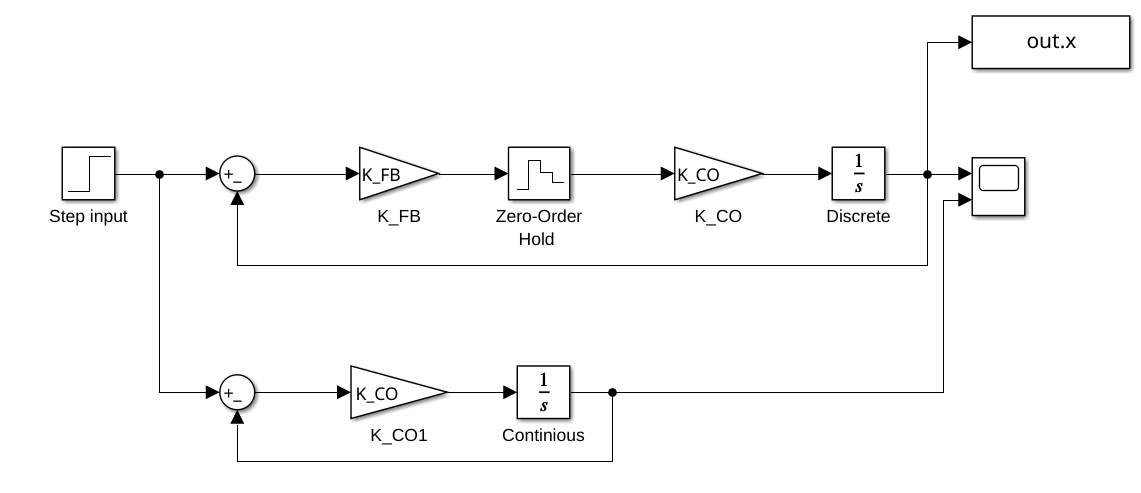
\includegraphics[width=\textwidth]{images/scheme_1.png}
    \caption{Схема 1.}
    \label{fig:scheme_1}
\end{figure}

Обозначим состояние системы за $x$. Очевидно, что $\dot{x}=0$ возможно только в случаях $K_{FB}=0$ или $x=1$. Первый случай соответствует нейтрольной границе устойчивости, второй --- устойчивому положению. Заметим также, что при $K_{FB}>\frac{2}{TK_{CO}}$ система теряет устойчивость (изменение переменной за период дискретизации превышает текущее расстояние до устойчивого положения в два раза, что приводит к нарастанию сигнала). При $K_{FB}=\frac{2}{TK_{CO}}=1.754$ достигается колебательная граница устойчивости.

При $K_{FB}>\frac{1}{TK_{CO}}$ система приобретает колебательность с периодом равным $T$ (максимальная аммплитуда --- на колебательной границе устойчивости). При $K_{FB}<\frac{1}{TK_{CO}}$ колебания отсутсвуют (изменение сигнала за время $T$ всегда меньше текущего расстояния до устойчивого положения). При $K_{FB}=\frac{1}{TK_{CO}}=0.877$ наблюдается наискорейший переходный процесс (за конечное время $T$).

Ниже приведены графики, демонстрирующие полученные свойства:
\begin{figure}
    [H]
    \centering
    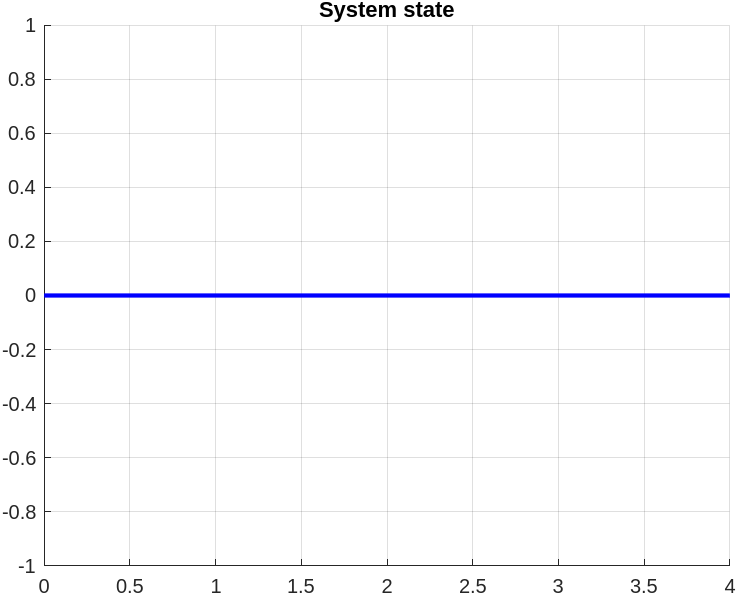
\includegraphics[width=350pt]{images/task1_b__neutral_state.png}
    \caption{Нейтральная грница устойчивости $K_{FE}=0$.}
\end{figure}
\begin{figure}
    [H]
    \centering
    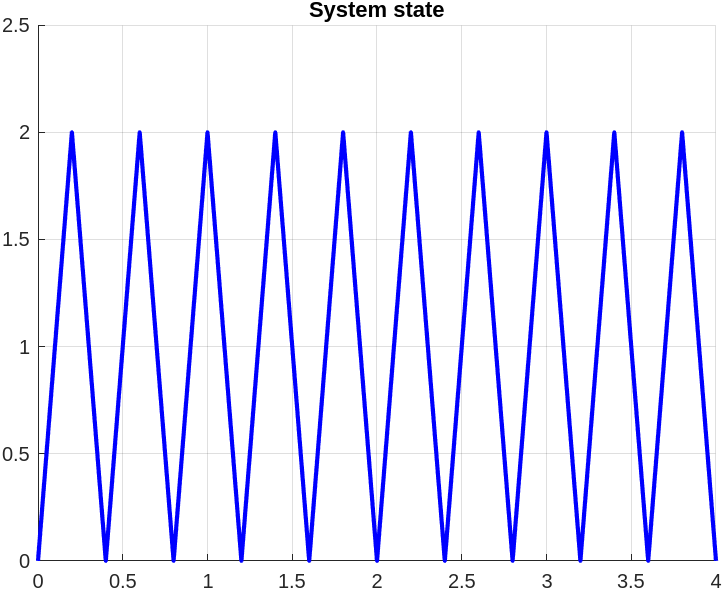
\includegraphics[width=350pt]{images/task1_b__oscill_state.png}
    \caption{Колебательная грница устойчивости $K_{FE}=1.754$.}
\end{figure}
\begin{figure}
    [H]
    \centering
    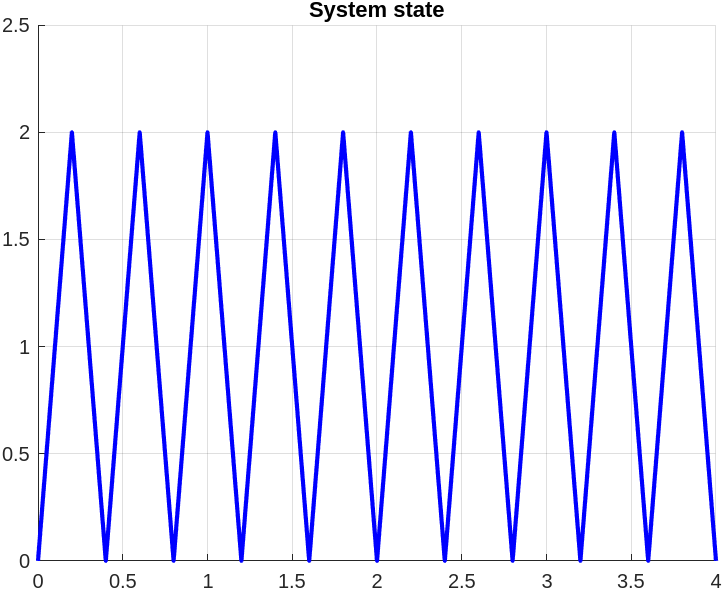
\includegraphics[width=350pt]{images/task1_d__max_state.png}
    \caption{Максимальная колебательность $K_{FE}=1.754$.}
\end{figure}
\begin{figure}
    [H]
    \centering
    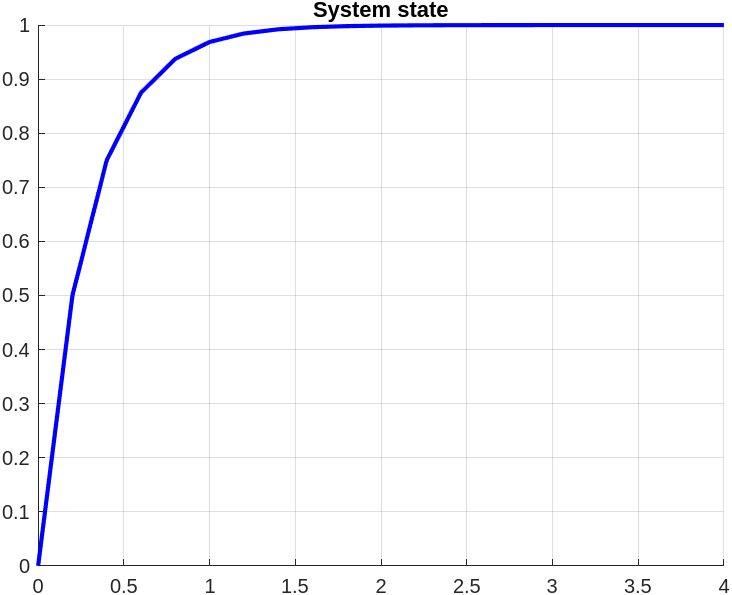
\includegraphics[width=350pt]{images/task1_d__no_state.png}
    \caption{Отсутствие колебаний $K_{FE}<0.877$.}
\end{figure}
\begin{figure}
    [H]
    \centering
    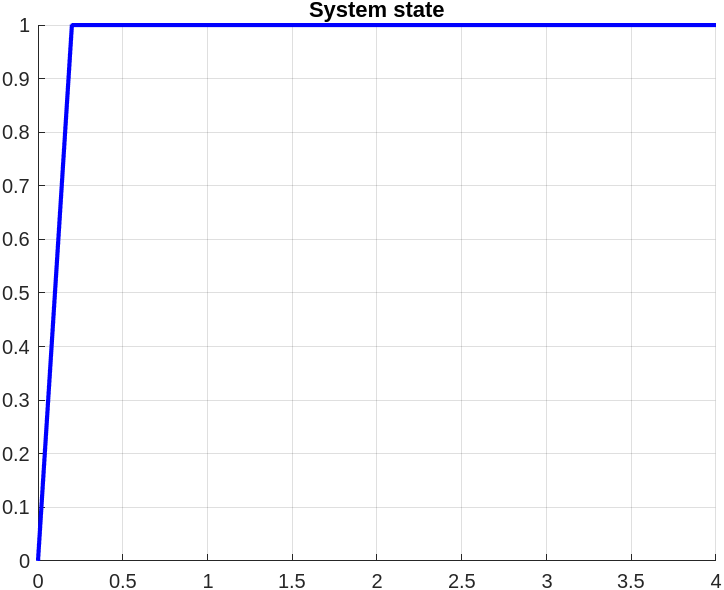
\includegraphics[width=350pt]{images/task1_e__optim_state.png}
    \caption{Оптимальное время переходного процесса ($T$) $K_{FE}=0.877$.}
\end{figure}

\subsection{Исследование устойчивости дискретных систем}
Рассмотрим непрерывную систему $\ddot{y} = u$:
\begin{equation}
	\begin{cases}
		\begin{bmatrix}
			\dot{x}_1 \\ \dot{x}_2
		\end{bmatrix} = 
		\begin{bmatrix}
			0 & 1 \\ 0 & 0
		\end{bmatrix}
		\begin{bmatrix}
			x_1 \\ x_2
		\end{bmatrix} + 
		\begin{bmatrix}
			0 \\ 1
		\end{bmatrix}u \\
		y = \begin{bmatrix}
			1 & 0
		\end{bmatrix} \begin{bmatrix}
			x_1 \\ x_2
		\end{bmatrix}
	\end{cases}
	\implies
	\begin{cases}
		\dot{x}=A_cx + B_cu \\
		y = Cx
	\end{cases}
\end{equation}

Воспользуемся выражениями \ref{eq:discr_sys} для дискретизации системы ($T=0.2$):
\begin{equation}
	\begin{cases}
		x(m+1) = Ax(m) + Bu(m)\\
		y(m) = Cx(m)
	\end{cases}, A = \begin{bmatrix}
		1 & 0.2 \\
		0 & 1
	\end{bmatrix}, B = \begin{bmatrix}
		0.02 \\ 0.2
	\end{bmatrix}
\end{equation}

Задавшись сигналом управления $u = -Kx$, можем добиться требуемых собственных чисел матрицы динамики системы $F = A-BK= \\=\begin{bmatrix}
	1 - 0.02k_1 & 0.2 - 0.02k_2 \\ -0.2k_1 & 1 -0.2k_2
\end{bmatrix}$ (модальный регулятор).

Для всех предложенных наборов корней выполнено условие $|z_i| < 1$ и все системы являются устойчивыми (что согласуется с корневым критерием, и также демонстрирует его применимость с комплексными корнями). 

Схема моделирования:
\begin{figure}
    [H]
    \centering
    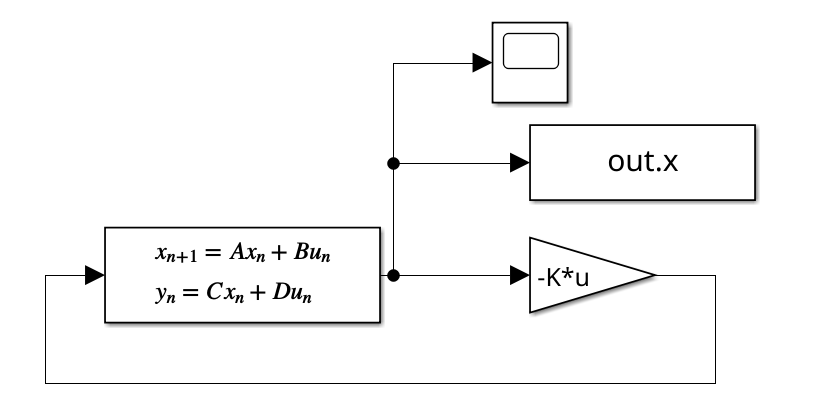
\includegraphics[width=350pt]{images/scheme_2.png}
    \caption{Схема 2.}
\end{figure}

Результаты моделирования представлены ниже:
\begin{figure}
    [H]
    \centering
    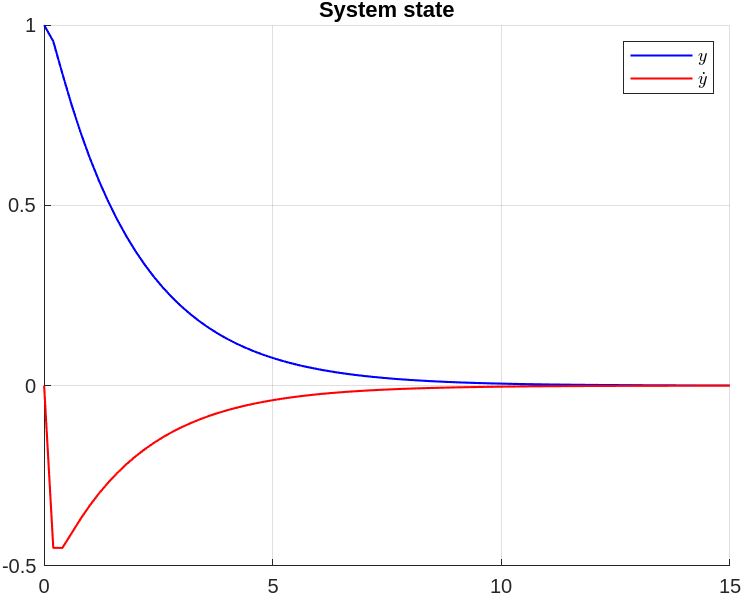
\includegraphics[width=350pt]{images/task2_d__1_state.png}
    \caption{Результат моделирования замкнутой системы ($z_1=0.9, z_2=0.1$).}
\end{figure}
\begin{figure}
    [H]
    \centering
    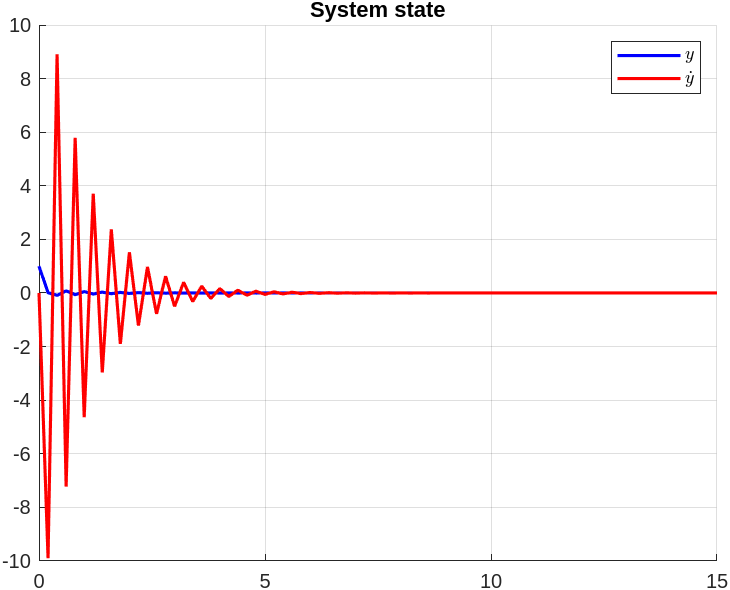
\includegraphics[width=350pt]{images/task2_d__2_state.png}
    \caption{Результат моделирования замкнутой системы ($z_1=-0.1, z_2=-0.8$).}
\end{figure}
\begin{figure}
    [H]
    \centering
    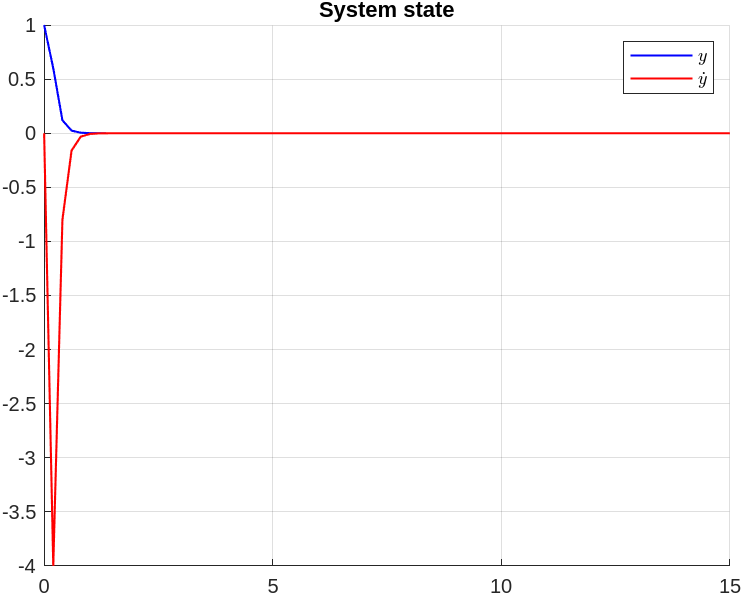
\includegraphics[width=350pt]{images/task2_d__3_state.png}
    \caption{Результат моделирования замкнутой системы ($z_1=0.2, z_2=0$).}
\end{figure}
\begin{figure}
    [H]
    \centering
    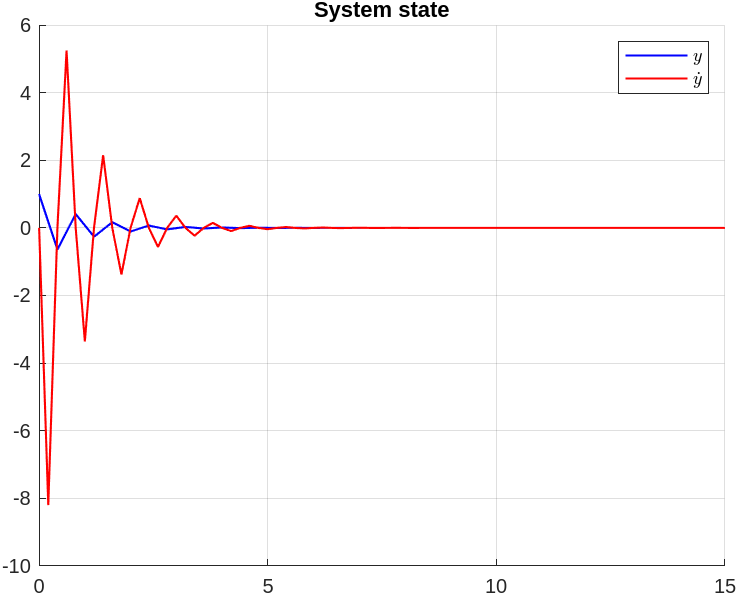
\includegraphics[width=350pt]{images/task2_d__4_state.png}
    \caption{Результат моделирования замкнутой системы ($z_1=0.8i, z_2=-0.8i$).}
\end{figure}
\begin{figure}
    [H]
    \centering
    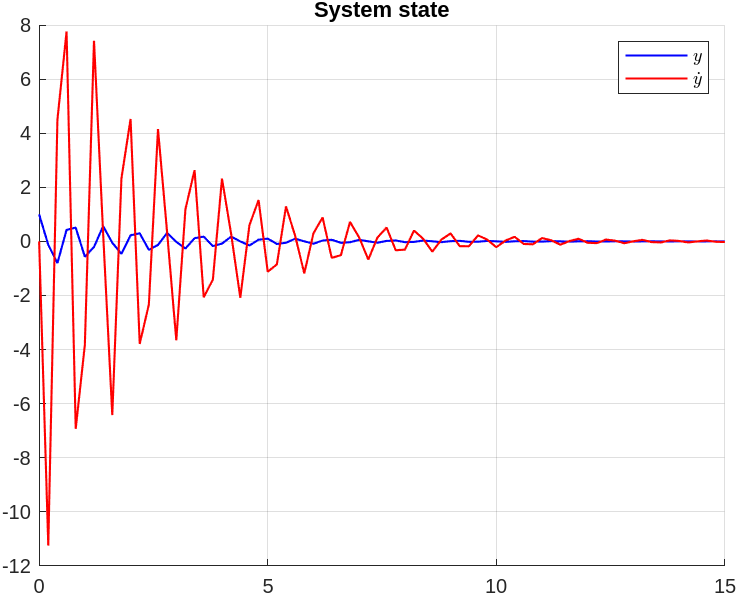
\includegraphics[width=350pt]{images/task2_d__5_state.png}
    \caption{Результат моделирования замкнутой системы ($z_1=-0.2+0.9i, z_2=-0.2-0.9i$).}
\end{figure}

\subsection{Построение дискретных командных генераторов}
Синтез требуемых командных генераторов приведен в качестве примеров в теоретической части (\ref{eq:gen1_sys} и \ref{eq:gen2_sys}). Построим схему для моделирования:
\begin{figure}
    [H]
    \centering
    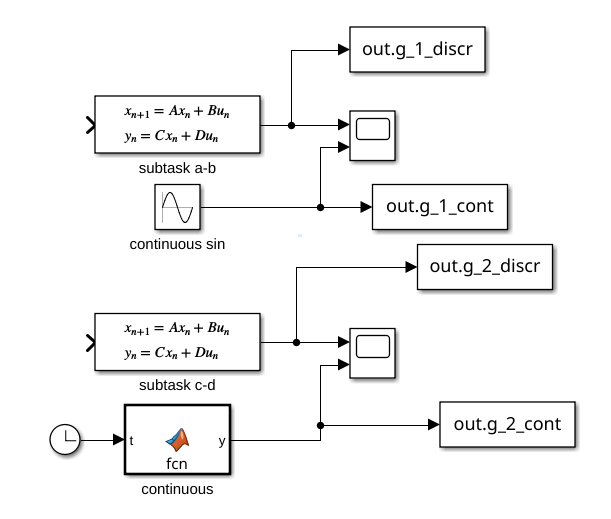
\includegraphics[width=350pt]{images/scheme_3.png}
    \caption{Схема 3.}
\end{figure}

Проведем моделирование, сравнив сигнал с непрерывным аналогом:
\begin{figure}
    [H]
    \centering
    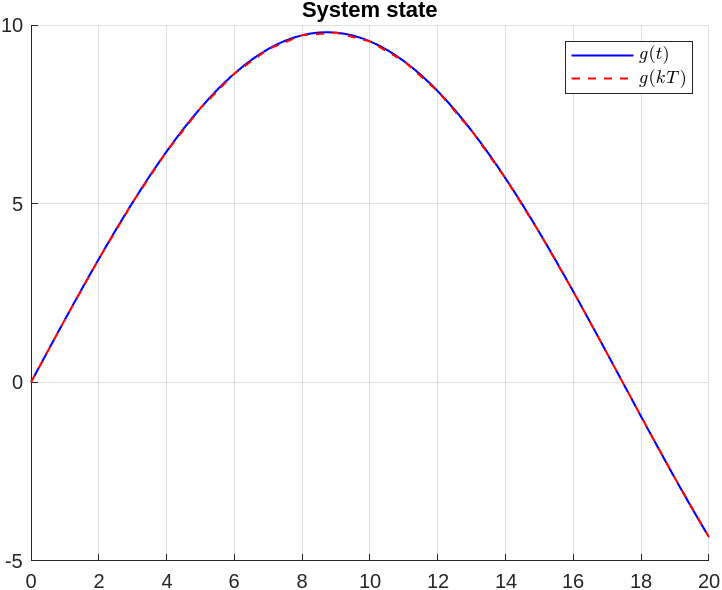
\includegraphics[width=350pt]{images/task3_state_1.png}
    \caption{Командный генератор гармонического сигнала \ref{eq:gen1}.}
\end{figure}
\begin{figure}
    [H]
    \centering
    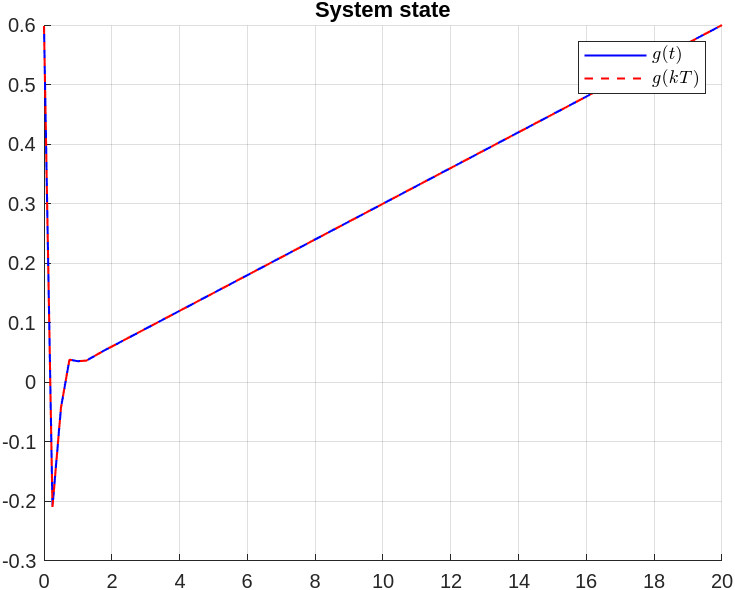
\includegraphics[width=350pt]{images/task3_state_2.png}
    \caption{Командный генератор сигнала \ref{eq:gen2}.}
\end{figure}

\section{Выводы}
В ходе выполнения работы ознакомились с принципом синтеза дискретных систем, анализом устойчивости, а также управления ими. Теоретические выкладки, сделанные в соответствующей секции были подтверждены во время про ведения экспериментов, что можно наблюдать на графиках моделирования.

\end{document}